\chapter{Transitivity parsing: the semantics}
\label{ch:semantic-parsing}

Semantic Role Labeling (SRL) is a well established task in the mainstream computational linguistics. Transitivity analysis is the SFL counterpart for SRL and constitutes the focus of this chapter. 

The general approach is to first account for covert syntactic constituents and after assign process types and participant roles according to a given resource. In current case the account for empty constituents is implemented as described in Government and Binding Theory (GBT) \citep{Haegeman1991} and the employed verb database is called Process Type Database (PTDB) \citep{Neale2002}. 

Compared to SRL task, where the majority of implementations use probabilistic models trained on an annotated corpus, I employ a static data base based on which I assign a set of configurations that may be the case, or what are the possibilities, rather than the best single guess. For this reason I use the preparatory step of identifying covert constituents (i.e. Null Elements) which reduces the number of possible assignments taking the analysis close to the goal of a single ``correct'' configuration.

\section{Creation of Empty Elements}
\label{sec:creation-empty-elements}
Sometimes a semantic participant is not mentioned (is elided) in a clause. It happens for one of two reasons: the participant mentions are contextually implicit and usually located outside the clause borders. So when they are implicit the resolution is contextual and required discourse structure awareness. This task is out of the current scope and constitutes a research field on its own. 

However, when the participants are missing because they are syntactically recoverable in the sentence then they are inferred from the structure and reference nodes are created for the missing elements. This phenomena are described in GB theory specifically the \textit{Control and Binding} of empty elements \citep{Haegeman1991} which has been introduced in Section \ref{sec:null-elements-gbt}. The \textit{reference constituents} are important for increasing the completeness of semantic analysis by making the participants and their afferent label explicit.

This stage is particularly important for semantic role labeling because usually the missing elements are participant roles (theta roles) shaping the semantic configuration. The most frequent are the cases of \textit{control} where the understood subject of a clause is in the parent clause like in examples \ref{ex:ctrl1} \ref{ex:ctrl3} where \textit{Subj} is a pronominal subject placeholder.
\begin{exe}
	\ex\label{ex:ctrl1}Piotr is considering whether [\textit{Subj} to abandon the investigation].
	\ex\label{ex:ctrl2}Susan promised us [\textit{Subj} to help].
	\ex\label{ex:ctrl3}They told you [\textit{Subj} to support the effort].
\end{exe}

There are also movement cases when a clause constituent receives no thematic role in higher clause but one in lower clause. The other case is of the non-overt constituents that are subjects in relative clauses and refer to head of the nominal group. This part of the algorithm is set up to detect cases of \textit{null elements} as described in the Chapter {ch:gbt} and create placeholder constituents for them which are in the next step enriched with semantic roles.

In Section \ref{sec:placing-null-elements} I discuss how to relate GBT to Stanford Dependency Grammar. This section discusses how to relate GBT to Systemic Functional Grammar. Currently the NP traces and PRO subjects are created with a set of graph patterns while the Wh traces are created with an algorithm.

\subsection{The PRO and NP-Trance Subjects}
The \textit{xcomp} relation in DC can be encoded as an CG pattern graph (Figure \ref{fig:arb-control}) targeting the constituents that are non-finite clauses functioning as complement that have no subject constituent of their own and no ``if'' and ``for'' markers (according to generalization \ref{gen:4}). They shall receive a the PRO subject constituent (governed or not) by the parent clause subject.

\begin{figure}[!ht]
	\centering
	\begin{tikzpicture}[tree-style] 
	\node[pattern-node, anchor=center] (vb1){class:clause}
	%child {node[pattern-node] (subj1) {class:nominal,\\element:subject,\\id:subj1}}
	child {node[pattern-node,below = 2em of vb1,] (vb2) {element:complement,\\class:clause,\\finiteness:non-finite}
		child {node[pattern-node-negative] (marker) {element:marker,\\words:[if,for]}}
		child {node[pattern-node-negative] (subj2) {element:subject,\\operation:insert}}
	};
	\end{tikzpicture}
	\caption{CG pattern for detecting PRO subjects}
	\label{fig:arb-control}
\end{figure}

The generalization \ref{gen:11} reflects criteria for selecting the controller of PRO based on its proximity in the higher clause. The schematic representation of the pattern for obligatory and subject object control is depicted in Figure \ref{fig:obj-control} and respectively \ref{fig:subj-control}. Please note that in case of Figure \ref{fig:subj-control} the prepositional complements do not affect subject control in any way since it specifies only the nominal complements this making it complementary to \ref{fig:obj-control} with respect to prepositional complements. 

\begin{figure}[H]
	\centering
	\begin{tikzpicture}[tree-style] 
	\node[pattern-node, anchor=center] (vb1){class:clause}
	child {node[pattern-node] (subj1) {class:nominal,\\element:subject}}
	child {node[pattern-node] (subj1) {class:nominal,\\element:complement,\\id:compl1}}
	child {node[pattern-node] (vb2) {class:clause,\\element:complement,\\finiteness:non-finite}
		child {node[pattern-node-negative] (marker) {element:marker,\\words:[if,for]}}
		child {node[pattern-node-negative] (subj2) {element:subject,\\operation:insert,\\arg:\{id:compl1\}}}
	};
	\end{tikzpicture}
	\caption{CG pattern for obligatory object control in complement clauses}
	\label{fig:obj-control}
\end{figure}

\begin{figure}[H]
	\centering
	\begin{tikzpicture}[tree-style] 
	\node[pattern-node, anchor=center] (vb1){class:clause}
	child {node[pattern-node] (subj1) {class:nominal,\\element:subject,\\id:subj1}}
	child {node[pattern-node-negative] (subj1) {class:nominal,\\element:complement}}
	child {node[pattern-node] (vb2) {class:clause,\\element:complement,\\finiteness:non-finite}
		child {node[pattern-node-negative] (marker) {element:marker,\\words:[if,for]}}
		child {node[pattern-node-negative] (subj2) {element:subject,\\operation:insert,\\arg:\{id:subj1\}}}
	};
	\end{tikzpicture}
	\caption{CG pattern for obligatory subject control in complement clauses}
	\label{fig:subj-control}
\end{figure}

In dependency grammar the adjunct clauses are also introduced via \textit{xcomp} and \textit{prepc} relations, so syntactically there is not distinction between the two and patterns from Figures \ref{fig:obj-control} and \ref{fig:subj-control} are applicable.

According to generalization \ref{gen:9} the PRO is optionally controlled in subject non-finite clauses. Since it is not possible to bind PRO solely on syntactic grounds in the generalization \ref{gen:9} is proposed the arbitrary interpretation.

\begin{figure}[H]
	\centering
	\begin{tikzpicture}[tree-style] 
	\node[pattern-node, anchor=center] (vb1){class:clause}
	%	child {node[pattern-node] (subj1) {class:nominal,\\element:subject,\\id:subj1}}
	%	child {node[pattern-node-negative] (subj1) {class:nominal,\\element:complement}}
	child {node[pattern-node, below =2em of vb1, anchor=north] (vb2) {class:clause,\\element:subject,\\finiteness:non-finite}
		child {node[pattern-node-negative, below =2em of vb2, anchor=north] (subj2) {element:subject,\\operation:insert,\\arg:\{words:one\}}}
	};
	\end{tikzpicture}
	\caption{CG pattern for arbitrary control in subject clauses}
	\label{fig:subj-arbitrary-control}
\end{figure}

The pattern for subject control in subject clause  is represented in Figure \ref{fig:subj-arbitrary-control}. This of course is an oversimplification and more rigorous binding rules can be be developed in a future work to cover binding scenarios exemplified in \ref{ex:pro12}-\ref{ex:pro15}.

\subsection{Wh-trances}

Creating constituents corresponding to Wh-traces involved a slightly larger number of scenarios and for the pragmatic reasons I have implemented the following algorithm rather than create the set of corresponding graph patterns. Nevertheless in the future this shall be expressed as graph patterns to be consistent with the general approach. The algorithm pseudo-code below shows how it is done. 

%\todo{Reformat the wh-trace algorithm}
%\todo{Remove function definition}

\begin{algorithm}[H]
	\Input { \dg, \cg}
	\Begin{
		\For {\Element \KwTo list of Wh-elements in entire \cg}
			{
				identify the Wh-groups containing the \Element\;
				identify the syntactic function of the Wh-element within the group\;
				identify the function of Wh-group in the clause\;
				check the number of clauses and which of clauses contains the Wh-group\;
				\If {more than one clause in \cg}
					{
						\For(low to high){\Group \KwTo \cg}
							{\If{Wh-group is \textbf{not} Subject \textbf{AND}\\ Wh-group is \textbf{not} in lowest embedded clause}
								{
								\eIf{Wh-group is Adjunct function}
								{create Adjunct Wh-trace using \dg and \cg}
								{create Theta Wh-trance using \dg and \cg}
								}
							}	
					}
			}
	}
	\caption{Creating the Wh-traces}
	\label{alg:create-wh-trace}
\end{algorithm}


\begin{algorithm}[!ht]
	\Input {\whGroup, \dg, \cg}
	\Begin{
		check the tense and modality for all the clauses\;
		\For(from the clause of \whGroup to lowest){$clause$ \KwTo \cg}
		{
			\tcc{create the adjunct trace in the first clause that has non present simple tense}
			\If{clause tense is \textbf{not} present simple}
			{
				create Adjunct Wh-trace for Wh-group\;
				\Return
			}
		}  
	}
	\caption{Creating the Adjunct (circumstantial) Wh-traces}
	\label{alg:create-wh-adjunct-trace}
\end{algorithm}



\begin{algorithm}[H]
	\Input {\whGroup, \dg, \cg}
	\Begin{
		get possible configurations for each clause from the PTDB\;
		\tcc{check if the higher clause is a projection and and has an extra argument}
		\ForEach{$config$ in higher clause configurations}
		{\If{ ($config$ is two role cognition \textbf{and} $config$ takes expletive subject) \textbf{or} ($config$ is three role cognition \textbf{and} $clause$ is passive voice)}
			{
				higher is eligible $\leftarrow$ True\;
				\textbf{break}\;
			}
		}
		\tcc{check if the lower clauses might miss an argument}
		\ForEach{$clause$ in lower clauses}
		{
			\ForEach{$config$ in clause configurations}
			{\If{number of clause theta constituents $ < $ number of config arguments}
				{
					lower is eligible $\leftarrow$ True\;
					break\;
				}
			}
		}
		\If{higher is eligible \textbf{and} lower is eligible}
		{
			\eIf{higher clause has ``that'' complementizer}
			{create Object Wh-trace in the lowest clause}
			% no there complementizer
			{\eIf {Wh-group has case}
				{
					\eIf{Wh-group case is nominative(subjective)}	 
					{create Subject Wh-trace in lowest clause}
					{create Object Wh-trace in lowest clause}
				}
				% no case
				{
					create Wh-trace with Subject function and attempt to assign theta roles\;
					\If{theta roles \textbf{not} successfully assigned in lower clause}
					{change the Wh-trace to Object function and assign theta roles}
				}
			}
		}
	}
	\caption{Creating the Theta (participant) Wh-traces}
	\label{alg:create-wh-theta-trace}
\end{algorithm}
\todo{Discuss the wh trace creation algorithm}

After the null elements are created the constituency graph is ready for the semantic enrichment stage semantic configuration are assigned to each clause. It is described in the next section.

\section{Semantic enrichment stage}
\label{sec:semantic-parsing}

In this section is explained how the parser assigns Transitivity configurations to the constituency graph. Transitivity roughly corresponds to what is known in computational linguistics as semantic analysis of text or \textit{semantic role labeling}. In this task the clause is assigned a semantic frame called configuration in which predicate functions as the process and the participants take frame dependent roles (or functions). The nodes that do not receive any participant role are the adjuncts which act as circumstances.

Because the proposed task goes beyond the syntactic structure it needs to rely on additional external semantic resources. One such resource is the Process Type Database(PTDB) created by \citet{Neale2002}. It is a table which listing possible configurations of semantic roles for each verb sense for over five thousands most popular verbs in English. This resource is then integrated into the current parser pipeline to automatically assignment semantic configurations and participant soles. How this is done is covered in the 

In the following I will explain the the practical steps of generating Transitivity but not before introducing the PTDB. Then I explain how the automation of the semantic role labeling is performed and why it is important to identify and create references to empty elements. 
%end chapter introduction

\subsection{The Process Type Database}
\label{sec:ptdb-description-technical}
The Process Type Database (PTDB) \citep{Neale2002} is the key resource in the automatization of Transitivity Analysis. It is the source for creating a set of graph patterns which are then used to enrich the constituency graph as described in the Section \ref{sec:enrichment-stage}. 

PTDB provides information on what possible process types and participants can correspond to a particular verb meaning. The PTDB is a dictionary-like dataset of verbs bound to an exhaustive list of verb senses and the corresponding Process Configuration for each of them.

In her work on PTDB \citet{Neale2002} improved the TRANSITIVITY system of the Cardiff Grammar by systematizing over 5400 senses (and process configurations) for  2750 most popular English verbs. Table \ref{tab:example-ptdb} presents a simplified sample of PTDB content.

\begin{table}[!ht]
	\centering
	\begin{tabulary}{\textwidth}{|C|C|c|c|}
		\hline
		\textbf{verb form} & \textbf{informal meaning} & \textbf{process type} & \textbf{configuration} \\ \hline
		calculate & work out by mathematics (commission will then,calculate the number of casted votes) & cognition & Ag-Cog + Ph \\ \hline
		& plan (newspaper articles were calculated to sway reader's opinions) & two role action & Ag + Cre \\ \hline
		catch & run after and seize (a leopard unable to catch its normal prey) & possessive & Ag-Ca + Af-Pos \\ \hline
		& fall ill (did you catch a cold?) & possessive & Ag-Ca + Af-Pos \\ \hline
		catch (up with) & reach (Simon tried to catch up with others) & two role action & Ag + Ra \\ \hline
	\end{tabulary}
	\caption{An example of records ins PTDB}
	\label{tab:example-ptdb}
\end{table}

\subsection{Cleaning up the PTDB}
The original version of the PTDB available on Neale's personal page is not usable for computational purposes as such. It  contains records applying a couple of different notation notations and sometimes informal, human friendly comments which represent noise for the computer programs and cannot be processed as such. In this section I explain now how the original PTDB was transformed in order to be used as a parsing resource.     

I focus on three columns which are of interest for the parsing purpose: the \textit{verb form} (1^{st}), the Cardiff grammar \textit{process type} (6^{th}) and the participant role \textit{configuration} (8^{th}) columns. Note that column numbers correspond to the original PTDB structure. 

After the transformation the PTDB column descriptions are as described in the Table \ref{tab:ptdb-comparison}. 
\begin{table}[]
	\centering
	\begin{tabulary}{\textwidth}{|l|L|L|}
		\hline
		\textbf{Column} & \textbf{Original}                    & \textbf{Modified}                                         \\ \hline
		1/A             & Form                                 & Form                                                      \\ \hline
		2/B    & \textit{Occurences of form}          & \textit{Occurences of form}                               \\ \hline
		3/C             & COB class (\& figure where possible) & COB class (\& figure where possible)                      \\ \hline
		4/D             & meaning descrition                   & meaning descrition                                        \\ \hline
		5/E             & Occurences in 5 million words        & Occurences in 5 million words                             \\ \hline
		6/F    & \textit{Cardiff Grammar feature}     & \textit{Cardiff Grammar process type (reindexed/renamed)} \\ \hline
		7/G             & Levin Feature                        & \textit{Cardiff participant feature}                      \\ \hline
		8/H             & \textit{Participant Role Configuration}       & \textit{Cardiff participant feature (extra)}              \\ \hline
		9/I             & Notes                                & Levin feature                                             \\ \hline
		10/J            &                                      & \textit{Participant Role Configuration}                   \\ \hline
		11/K            &                                      & Notes                                                     \\ \hline
	\end{tabulary}
	\caption{The table structure of PTDB before and after the transformation}
	\label{tab:ptdb-comparison}
\end{table}

Next I describe the transformed PTDB and how it be interpreted. For a start, the verb form column contains either base form of the verb (e.g. draw, take), base form plus a preposition (e.g. draw into, draw away, take apart, take away from) or base form plus a phraseologic expression (e.g draw to an end, take on board, take the view that, take a shower). The prepositions are either the verbal particles or the preposition introducing the prepositional phrase complement. Prepositions often influence the process type and the participant configuration. So they are good cues to be considered during the semantic role assignment. The verb forms that have the same process type and configuration but different prepositions often are grouped together delimited by a slash ``/'' (e.g. draw into/around, take off/on) or if optional (i.e. coincide with the meaning of the verb base form without any preposition) they are placed in round brackets ``()'' (e.g. flow (into/out/down) ).

The process type column registers one feature in the PROCESS-TYPE systemic network depicted in Figure \ref{fig:transitivity-system}. 

The participant configuration column contains the sequence of participant type abbreviations joined by plus sign ``+'' (e.g. Ag + Af, Em + Ph, Ag-Cog + Ph). The order of participants corresponds to the Active voice in Declarative mood also called the \textit{canonical form of a configuration}. Originally the configurations contained the ``Pro'' abbreviation signifying the place of the main verb/process. As all configurations are in canonical form, the Pro was redundant occurring always in the second position thus had been removed. So the first participant corresponds to the Subject, second to the first complement and third to the second complement. Some participants are optional for the meaning and are marked round brackets ``()'' (e.g. Ag + Af-Ca (+ Des) ) meaning that the participant may or may not be realized.

Not all the records in the original resource fulfill the description above and needed corrections. For example when Neale had doubts during the making of PTDB, she marked uncertainties with question mark ``?''. Commas ``,'' and and ``\&'' sign are use with various meaning and inconsistently in all columns. Comments such as ``not in Cob'' were encountered across several columns. 

Some records contain only prepositions listed in the verb form column which actually represent omissions of the main verb which is to be found in the immediately preceding records(s), this have been fixed by pre-pending the verb form to the preposition. 

%The account of verb meanings in PTDB is not exhaustive. Compared to VerbNet or FrameNet there are considerably less meanings described. 

Among the identified verb meanings in PTDB, there are some that do not contain configurations. These records missing a process type and configuration had not been suppressed. 

The process type feature column contained originally a second feature which had been removed, representing a compressed version of the participant configuration however it was redundant as the full configuration is registered in the next column. 

In PTDB Neale uses a slightly different process type names than the ones adopted in this work. The process type features have been re-indexed and adapted to match exactly the feature labels in the PROCESS-TYPE systemic network (e.g. ``one role action'' became ``one-role-action''). Annexe \ref{ch:reindexing-ptdb} provides the mapping across the process type versions. 

Configuration column is one of the most important ones in PTDB. Checking it's consistency conform to Fawcett's Transitivity system revealed the need for some corrections. For example ``Af + Af'', ``Af-Ca + Pos + Ag'', ``Af-Cog + Ph + Ag'' are grammatically impossible configurations and were manually corrected to the closest likely configuration ``Ag + Af'', ``Ag + Af-Ca + Pos'', ``Ag + Af-Cog + Ph''.

Other records, judged by the process type, were incomplete. For example instances of two role action registered only one of the role e.g. Af or Ca omitting the Ag participant. These records have been also manually corrected by perpending the Ag, Ag-Af or Cog roles depending on the case. 

The ``Dir'' participant is interpreted as direction is not registered/defined in the Cardiff Grammar. Nevertheless there is a ``Des'' participant which I believe is the closest match. Therefore all ``Dir'' occurrences had been changed to ``Des''. One may argue that the two have different meanings however grammatically they seem to behave the same (at least in the accounted configurations). 

By contrast some process types had been changed from Action into either Locational or Directional because they contained either Loc (location), Des (destination) or So (source) participants which are not found in Action processes unless they function as Adjuncts which are out of the context of the current description.

A note worth making here is that the Locational, Movement specifically but also other spatial verbs are very difficult to assign roles correctly because their participants are Locations, Directions, Destinations etc. which can also serve as spatial adjuncts. This aspect has not been directly addressed in present work and is reflected by a lower accuracy for these classes of verbs. 

\begin{figure}[!ht]
	\centering
	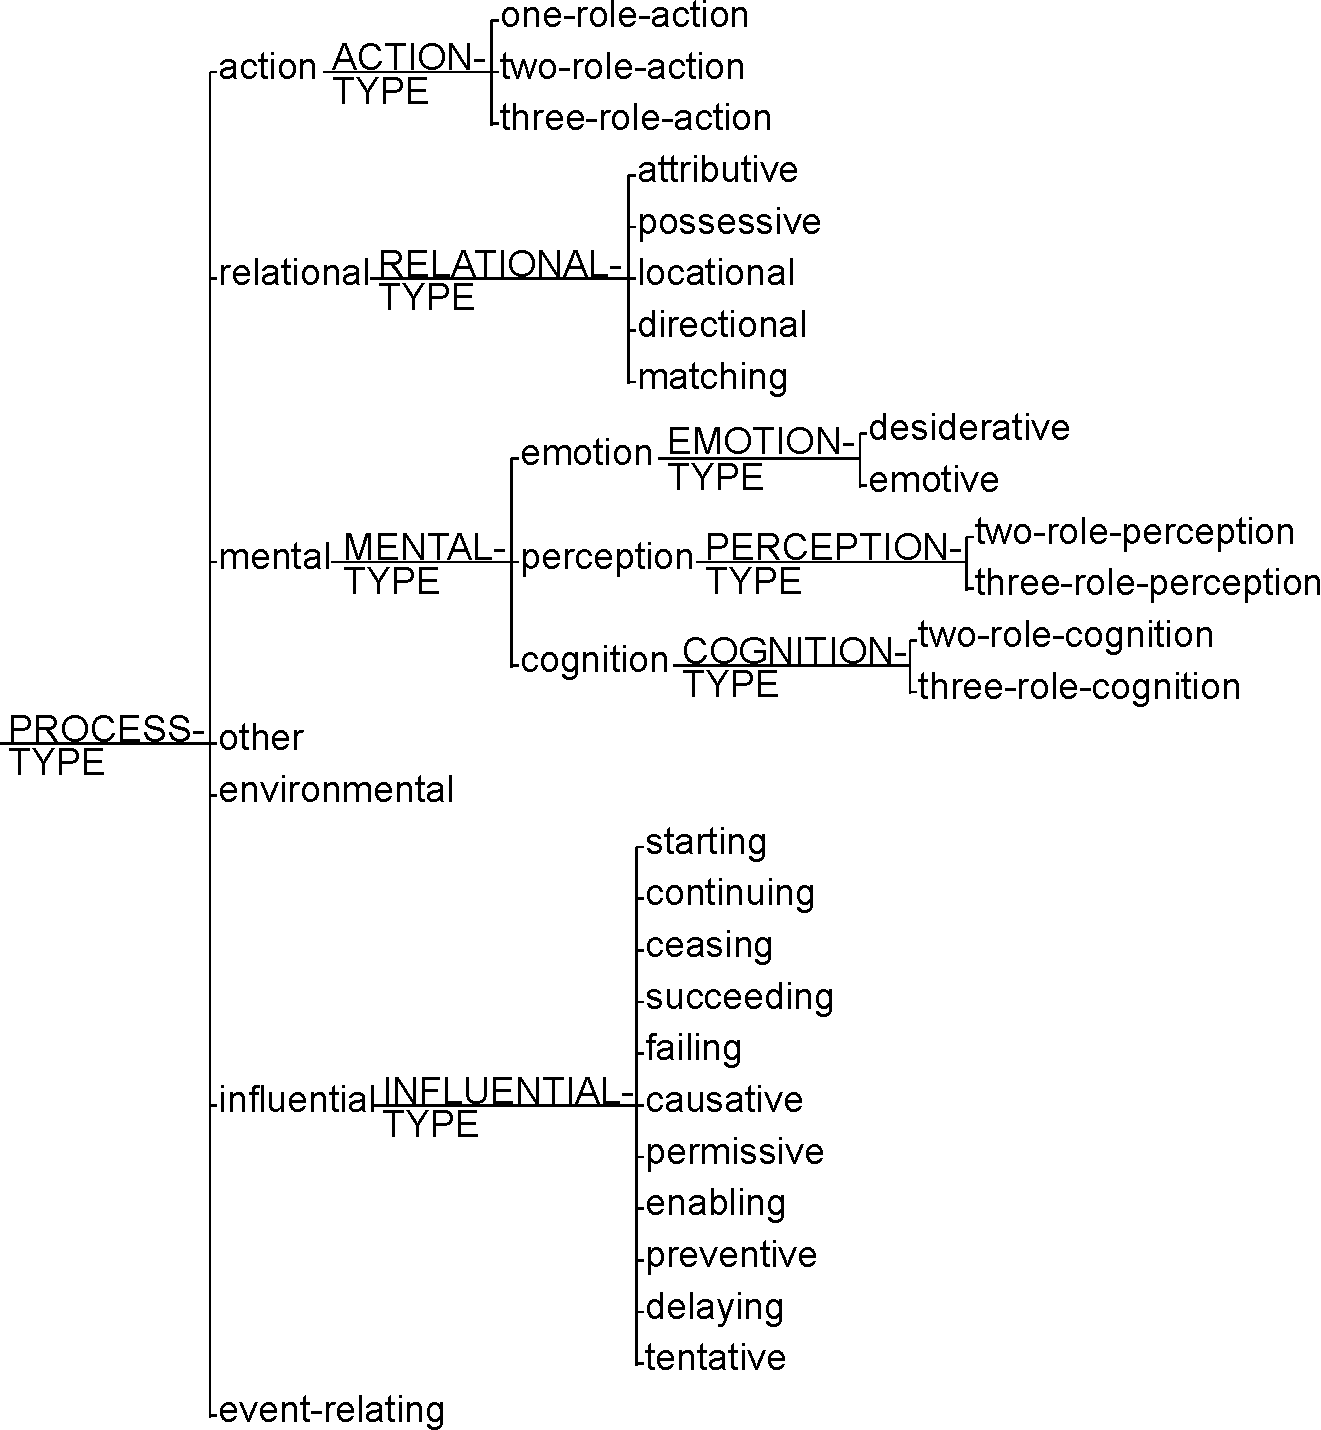
\includegraphics[width=0.7\linewidth]{Figures/SFL-grammar/Transitivity}
	\caption[Transitivity System in Cardiff Grammar]{Transitivity System in Cardiff Grammar}
	\label{fig:transitivity-system}
\end{figure}

The Cardiff features column indicates the process type selected in the TRANSITIVITY system corresponding to one of the top levels depicted in Figure \ref{fig:transitivity-system}

\subsection{Generation of the Configuration Graph Patterns}
\label{sec:gen-sem}
The configuration pattern graphs are used for CG enrichment executed through graph matching operation described in Section \ref{sec:pattern-graph-matching}. The PTDB has been cleaned up and normalized to support automatic generation of the \textit{Configuration Graph Patterns} (CGP). These graph patterns represent a constrained syntactic structure that carry semantic features. The latter are to be applied if the graph pattern is identified the sentence CG. 

CGPs are generated from the process type and participant configuration columns of the PTDB. Figure \ref{fig:general-configuration-canonic} depicts the prototypical template for generating three role CGP for canonic participant order (indicative mood active voice). This part assigns the Clause constituent Process Type (i.e. configuration type) while Subject and Complement constituents receive participant roles. 

\begin{figure}[H]
	\centering
	\begin{tikzpicture}[tree-style, level 1/.style={sibling distance=12em},] 
	\node[pattern-node, anchor=center] (proc){class:clause,\\mood:declarative,\\operation:update,\\ arg1:\{configuration:configuration-type\}}
	child{node[pattern-node]{element:subject,\\operation:update,\\ arg1:\{participant:Role1\}} edge from parent node[left] {}}
	child{node[pattern-node]{element:complement,\\operation:update,\\ arg1:\{participant:Role2\}} edge from parent node[below] {}}
	child{node[pattern-node]{element:complement,\\operation:update,\\ arg1:\{participant:Role3\}} edge from parent node[right] {}};
	\end{tikzpicture}
	\caption{Indicative mood and active voice configuration pattern with three participant roles}
	\label{fig:general-configuration-canonic}
\end{figure}

Besides the canonic CGP a set of variations are generated for each configurations by transforming the canonic configuration. The variations are function of the process type, participant roles, mood and voice. When each of the variants are supported by the process type and participant configuration the flowing CGP are generated: (1) the declarative
active (2) the passive (3) the imperative and (4) Wh-interrogative (Wh-Subj/Wh-obj/Wh-adj especially important for locational and directions processes).

%\explain{how do the process type influence the generated forms and also how the participant roles influence the forms?}
%\explain{How do the CGP vary according to other features such as voice and mood}
%\explain{What happens in Wh-Subj/Wh-obj/Wh-adj? what happens in Wh-YN, how are the patterns generated to cove those?}

If the configuration accepts passive voice i.e. the first configuration role is not expletive ``there'' or pleonastic ``it'' and the last role is not Agent role then both active and passive voice CPG are generated.

The imperative form CGP is generated if the first role of the configuration implies an active animate entity. Roles that accept imperative form are: Agent, Emoter, Cognizant, Perceiver and their compositional derivations (e.g. Agent-Carrier, Agent-Cognizant, Affected-Emoter etc.)

The passive differs from active voice pattern by switching places of the first two roles resulting in the second role matched to the subject function and the first role one the first complement. In the case of imperative the first role  as well as the subject constituent are simply omitted.  

Algorithm \ref{alg:generating-cpg} outlines how the CPGs are generated from the PTDB. The CPGs are represented as Python structures and are stored in a Python module. This way the graph patterns are accessible as native structures making it handy to instantiate the graph patterns. 


\begin{algorithm}[H]
	\Input { PTDB }
	\Begin{
		generate unique set of process type + participant roles\;
		generate unique set os process type\;
		\For{process type \KwTo possible process type}
		{
			generate configuration set for given process type \;
			\For{configuration \KwTo configuration set}
			{
				generate indicative active pattern graph \;
				\If {no expletive in configuration}
				{
					\If{configuration accepts passive}
					{
						generate indicative passive pattern graph\;
					}
					\If{configuration accepts imperative}
					{
						generate imperative pattern graph\;
					}
					\If{Locational process}
					{
					generate expletive there pattern graph \;
					}
					\If{configuration participants may function as Adjuncts}
					{
						\tcc{the Directional processes varying optional Source, Path and Destination}
						generate variate role indicative active pattern graphs \;
						generate variate role indicative passive pattern graphs \;
						generate variate role imperative pattern graphs \;
						generate variate role Wh-interrogative pattern graphs \;
					}
				}
			}
		}
	}
	\caption{Generating the CPGs from the PTDB}
	\label{alg:generating-cpg}
\end{algorithm}

The first two lines of the algorithm synthesize the PTDB by grouping unique configurations for each process type. Then for each configuration of each process type is generated one to three pattern graphs depending on the configuration and process type specifics.

\begin{figure}[H]
	\centering
	\begin{tikzpicture}[tree-style, level 1/.style={sibling distance=12em},] 
	\node[pattern-node, anchor=center] (proc){class:clause, \\operation:update,\\ arg1:\{process:Process-Type\}}
	child{node[pattern-node]{element:subject,\\operation:update,\\ arg1:\{participant:Role2\}} edge from parent node[left] {}}
	child{node[pattern-node]{element:complement,\\operation:update,\\ arg1:\{participant:Role1\}} edge from parent node[below] {}}
	child{node[pattern-node]{element:complement,\\operation:update,\\ arg1:\{participant:Role3\}} edge from parent node[right] {}};
	\end{tikzpicture}
	\caption{Indicative mood and passive voice configuration pattern with three participant roles}
	\label{fig:general-configuration-passive}
\end{figure}

\begin{figure}[H]
	\centering
	\begin{tikzpicture}[tree-style, level 1/.style={sibling distance=12em},] 
	\node[pattern-node, anchor=center] (proc){class:clause, \\operation:update,\\ arg1:\{process:Process-Type\}}
	child{node[pattern-node-negative]{element:subject} edge from parent node[left] {}}
	child{node[pattern-node]{element:complement,\\operation:update,\\ arg1:\{participant:Role2\}} edge from parent node[below] {}}
	child{node[pattern-node]{element:complement,\\operation:update,\\ arg1:\{participant:Role3\}} edge from parent node[right] {}};
	\end{tikzpicture}
	\caption{Imperative mood configuration pattern with three participant roles}
	\label{fig:general-configuration-imperative}
\end{figure}

%\todo{Explain the rules by which are created variations on voice, mood (and other features) based on configuration type and participants}
The indicative mood active voice pattern (depicted in Figure \ref{fig:general-configuration-canonic}) corresponding to the canonic form in PTDB is always generated. If the configuration does not contain an expletive and accepts passive voice then the corresponding pattern is generated with first and second roles switched like in Figure \ref{fig:general-configuration-passive}. If the configuration accepts imperatives then also a subjectless pattern graph is generated with first role omitted as depicted in Figure \ref{fig:general-configuration-imperative}. 

Directional processes are rather a special case. Examples \ref{ex:directional2} to \ref{ex:directional4} are equally valid configurations. Example \ref{ex:directional5} is a generic representation highlighting the optionality of these participants. 
%\todo{Discuss Neale/Fawcett possible configurations}
\begin{exe}
	\ex\label{ex:directional2} The parcel traveled from London[So].
	\ex\label{ex:directional3} The parcel traveled via Poland[Pa].
	\ex\label{ex:directional4} The parcel traveled to Moscow[Des].
	\ex\label{ex:directional5} The parcel traveled (from London[So]) (via Poland[Pa]) (to Moscow[Des]).
\end{exe}

So in Directional configurations second, third and fourth participants are optional and may occur in any order but at least one of them should be present. Therefore So, Pa and Des participants patterns should be generated for all combinations as presented in the Table \ref{tab:directional-partic-variations} below.

\begin{table}[H]
	\centering
	\begin{tabular}{|c|c|c|}
		\hline
		\textbf{So} & \textbf{Pa} & \textbf{Des} \\ \hline
		\textbf{+} & - & - \\ \hline
		- & \textbf{+} & - \\ \hline
		- & - & \textbf{+} \\ \hline
		\textbf{+} & \textbf{+} & - \\ \hline
		\textbf{+} & - & \textbf{+} \\ \hline
		- & \textbf{+} & \textbf{+} \\ \hline
		\textbf{+} & \textbf{+} & \textbf{+} \\ \hline
	\end{tabular}
	\caption{Participant arrangements for Directional processes (order independent)}
	\label{tab:directional-partic-variations}
\end{table}

Finally, the CPGs are grouped by process type. This alleviates the burden of selecting the number of patterns to test for a certain clause. The python structure looks as represented in Listing \ref{lst:config-pattern-set}

\begin{lstlisting}[language=json,firstnumber=1, caption={Configuration Pattern Set as a Python dictionary structure},label={lst:config-pattern-set}]
configuration_pattern_set = {
	process_type1 : {
		config1 : [pattern1, panttern2,...],
		config2 : [pattern3, panttern4,...],
	},
	process_type2 : {
		config3 : [pattern5, panttern6,...],
		config4 : [pattern7, panttern8,...],
	}
	...
}
\end{lstlisting}

\subsection{Transitivity parsing algorithm}
Transitivity enrichment is performed on the constituency graph after it has been enriched with Mood features and the null elements had been identified and appended. 


\begin{algorithm}[H]
	\Input { \cg, \dg }
	\Begin
	{
		\For{ clause \KwTo clauses in mcg}
		{
			select from PTDB candidate process types and configurations\;
			filter configurations fitting the clause \;
			\For{config \KwTo valid possible configurations}
			{
				filter pre-generated pattern graphs of the config fitting the clause\;
				\For{pattern \KwTo filtered pattern graph set}
				{
					\label{line:enrich-from-pattern} enrich clause using pattern and mcg filtered by role constraints\;
				}
			}
		}
	}
	\caption{Transitivity parsing}
	\label{alg:transitivity-parsing}
\end{algorithm}

Algorithm \ref{alg:transitivity-parsing} outlines the semantic parsing process implemented in the current parser which is a cascade of three loops. 

The first loop iterates through clauses in the mood constituency graph and for each the candidate process types are identified by considering: (a) the main verb, (b) the prepositions connected to it (either prepositional particles, or prepositions introducing a complement or adjunct prepositional phrase listed in Table \ref{tab:participant-roles-constraints}) or (c) phrasal expressions such as "take a shower" which are explained in Section \ref{sec:ptdb-description-technical}.

\begin{table}[]
	\centering
	\begin{tabular}{|l|l|}
		\hline
		\textbf{Role} & \textbf{Prepositions}             \\ \hline
		Des           & to,towards,at,on,in,              \\ \hline
		Ben           & to,for,                           \\ \hline
		Attr          & as,                               \\ \hline
		Ra            & on,in,                            \\ \hline
		So            & from,                             \\ \hline
		Pa            & through,via,                      \\ \hline
		Loc           & in,at,into,behind,in front of, on \\ \hline
		Mtch          & with,to,                          \\ \hline
		Ag            & by,                               \\ \hline
		Ph            & about,                            \\ \hline
		Cog           & to                                \\ \hline
	\end{tabular}
	\caption{Prepositional constraints on participant roles }
	\label{tab:participant-roles-constraints}
\end{table}


The second loop iterates through the candidate configurations for each candidate process type and selects the graph patterns that shall be matched to the current clause. Then iteratively, each of the retrieved graph patterns (in the third loop) are applied to the clause graph. Line \ref{line:enrich-from-pattern} enriches CG nodes with new features of the pattern graph each time they are successfully matched. 
Before enrichment the CG nodes are checked against an additional set of condition (captured by Algorithm \ref{alg:role-constraint-check}) which were omitted in the pattern graph. These conditions may prevent the enrichment even if the pattern has been identified. 

%\explain{What is the selection/filtering based on ? probably subj/role, preposition/role constraints} The last set of checks is an attempt to reduce the false positive assignments. 
%%For example if the complement is a clause then it can take only Phenomena role otherwise the entire

\begin{algorithm}[]
	\Input {\node, role, \dg }
	\Begin
	{
		\tcc{Cog, Em and Perc must be animates}
		\If{role is Cog \textbf{or} Em \textbf{or} Perc}
		{
			check that the \node has animate feature \;
		}
		\tcc{clauses can only be phenomenas}
		\If{\node is a clause}{
			check that role is Ph only \;
		}
		\tcc{prepositional phrases can only start with certain prepositions for a role}
		\If{\node is a Prepositional Phrase}
		{
			get the list of allowed prepositions for the role \;
			check if the prepositional phrase starts with any of the allowed prepositions \;
		}
	}
	\caption{Participant Role constraint check if a role is not illegal for constituent}
	\label{alg:role-constraint-check}
\end{algorithm}

The Transitivity parsing results in multiple process configurations being assigned to clauses introducing uncertainty. This uncertainty, laying within the reasonable limits, is not dealt with by the current parser but shall be further resolved through deeper semantic and pragmatic means. 

\section{Discussion}

This chapter describes how the semantic role labeling from Transitivity system network is performed on top of the constituency graph. 

First null elements are identified and filled with proxy constituents. This process ensures higher accuracy of semantic role assignments from the configuration patterns in the second step. 

The configuration patterns have been generated from the PTDB - a verb database accounting for Transitivity patterns in Cardiff grammar. In order to generate these patterns the PTDB had to be first cleaned up, unified and aligned to the present Transitivity system. Then for each configuration were generated a set of possible patterns varying based on mood, voice, process type and participants. 

Finally the semantic role labeling step employs the same pattern based enrichment mechanism as the one used in Section \ref{sec:enrichment-stage}

The Algorithms can be improved a great deal by externalization of constraints and conditions. Some of them however are too complex to check to be completely removed but in the next iterations the tendency should definitely be towards higher abstraction and separating the grammatic constraint as realization rules from the code. 
